\documentclass{article}
    \usepackage[UTF8]{ctex}
    \usepackage{caption}
    \usepackage{graphicx, subfig}


 \title{ 第二章. 概率复习}
 \begin{document}
 \date{}
 \maketitle
 \setcounter{section}{1}
  \section{概率}
   \subsection{概率}
   \begin{quote}
    概率论只不过是常识而已. -Pierre Laplace,1812
   \end{quote}
   在前一章中,我们看到了概率在机器学习中如何发挥作用。 
   在本章中,我们更详细地讨论概率论。 我们没空去做非常详尽的介绍 - 
   因此,您最好去看一些关于此主题的优秀教科书,例如(Jaynes 2003; Bertsekas和Tsitsiklis 2008; Wasserman 2004)。
   但是我们会简要回顾许多您将在后面的章节中需要的关键想法。
   \par
   在我们开始一些更有技术性的问题之前,让我们停下来并问问自己:什么是概率?
   我们都很熟悉,硬币正面朝上的概率是50\%,但是这究竟意味着什么呢?
   实际上对于概率有两种解释.其中一种是频率主义者的解释,在这个观点中
   ,概率代表着事件长期运行的频率.例如,如果我们抛很多次硬币,我们期望有一半的次数是正面朝上。
   \par
   另一种就是贝叶斯解释,在这个观点中,概率被用来量化我们对某事的不确定性;
   因此他跟我们得到的信息有着更基本的关系,而不是重复试验.在贝叶斯的观点中,
   上述的声明表示:我们相信下一次投硬币朝上和朝下的概率是相等的。
   \par
   贝叶斯解释的一大优势是,我们可以利用它对没有长期频率的事件的不确定性(uncertainty)建模模拟。
   例如,我们可能想要计算2020年前极地冰盖将会融化的概率。
   此事件将发生零次或一次,但不能重复发生。 
   尽管如此,我们应该能够量化我们对这个事件的不确定性。 
   根据我们认为的这个事件的可能性,我们将(希望是这样!)采取适当的行动
   (参见第5.7节讨论,如何在不确定情况下做出最优决策)。
   此外还有更多的机器学习方面的例子,比如我们可能会收到特定的电子邮件,并且想要计算它是垃圾邮件的概率。 或者我们可能在我们的雷达屏幕上观察到一个“昙花一现”的东西,并且想要计算相应目标(不管是鸟,飞机还是导弹)位置的概率分布。 在所有这些情况下,重复试验的想法没有意义,
   但贝叶斯解释在这种情况下是有效的,而且确实很自然.因此,我们将在本书中采用贝叶斯解释。 幸运的是,无论采用哪种解释,概率论的基本规则都是一样的。
   \begin{figure}
    \centering
    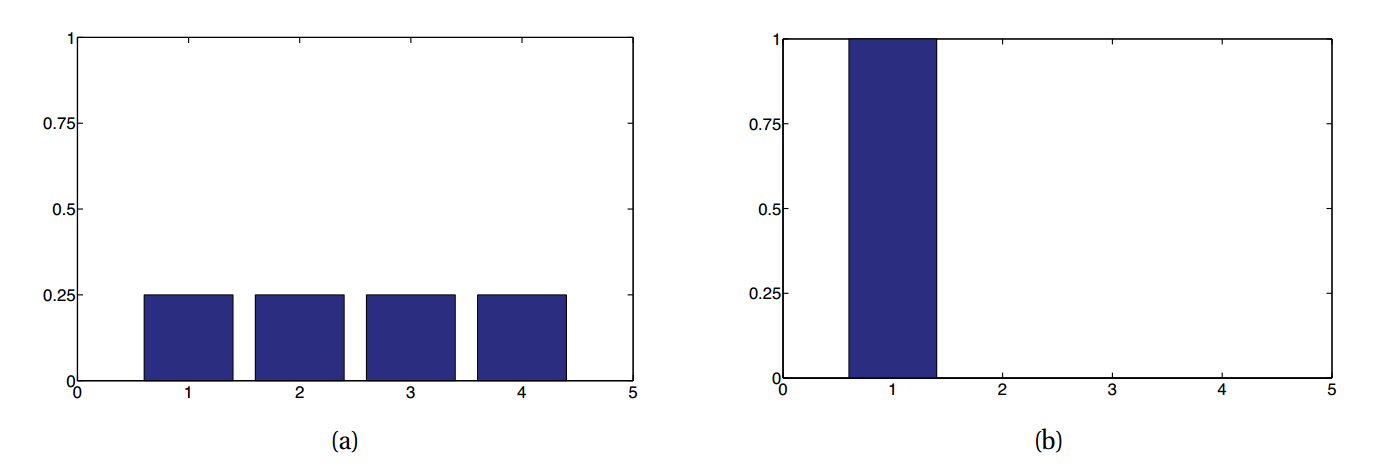
\includegraphics[width=.8\textwidth]{./Picture/21.png} %1.png是图片文件的相对路径
    \caption*{2.1 a:均匀分布 b:退化分布} %caption是图片的标题
    \label{img1} %此处的label相当于一个图片的专属标志,目的是方便上下文的引用
  \end{figure}
  \subsection{概率论简要复习}
  本节简要回顾了概率论的基础知识,仅仅是对可能“大脑记忆生锈”的读者的复习。 
  已经熟悉这些基础知识的读者可以地跳过本节。
  \subsubsection{离散随机变量}
  \subsubsection{基本规则}
  \subsection{一些常见的离散变量分布}
  \subsection{一些常见的了连续变量分布}
  \subsection{联合概率分布}
  \subsection{随机变量的变换(Transformations)}
  \subsection{蒙特卡洛近似}
  \subsection{信息论}
  \subsection*{习题}
\end{document}
